% !TeX root = ../main.tex

\newlecture[Dynamic Programming][Nov 2, 2026]

\header{Running Present Value}
A \dbb{recursive} method for calculating present value. Let
\[PV(i) = \text{present value (at time } i\text{) of all cash flows occurring at time } i \text{ and later.}\]
Start at the \ul{end} and work backwards, discounting one period at a time with the forward short rates:

\begin{center}
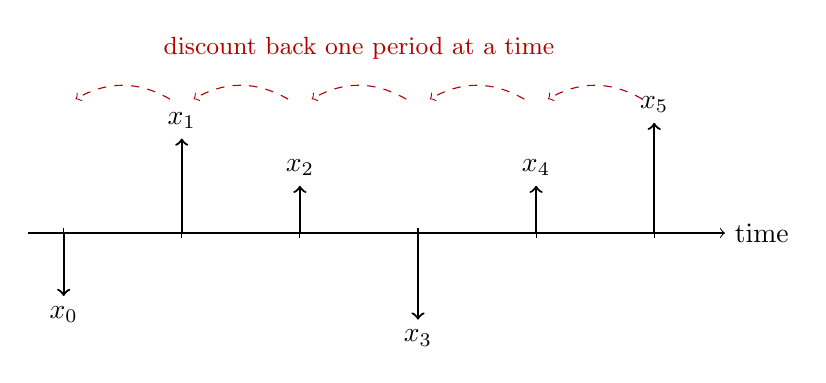
\begin{tikzpicture}[x=1.5cm]
    \draw[->] (-0.3,0) -- (5.6,0) node[right] {time};
    \foreach \x in {0,...,5} { \draw (\x,0.06) -- (\x,-0.06); }
    \draw[->, thick] (0,0) -- (0,-0.8) node[below] {$x_0$};
    \draw[->, thick] (1,0) -- (1,1.2) node[above] {$x_1$};
    \draw[->, thick] (2,0) -- (2,0.6) node[above] {$x_2$};
    \draw[->, thick] (3,0) -- (3,-1.1) node[below] {$x_3$};
    \draw[->, thick] (4,0) -- (4,0.6) node[above] {$x_4$};
    \draw[->, thick] (5,0) -- (5,1.4) node[above] {$x_5$};
    \foreach \x in {5,4,3,2,1} {
        \draw[->, red!70!black, dashed] (\x-0.1,1.7) to[bend right=30] (\x-0.9,1.7);
    }
    \node[red!70!black] at (2.5,2.35) {\small discount back one period at a time};
\end{tikzpicture}
\end{center}

\[\begin{aligned}
    PV(5) &= x_5\\
    PV(4) &= x_4 + \frac{PV(5)}{1+f_{4,5}}\\
    PV(3) &= x_3 + \frac{PV(4)}{1+f_{3,4}}\\
    PV(2) &= x_2 + \frac{PV(3)}{1+f_{2,3}}\\
    PV(1) &= x_1 + \frac{PV(2)}{1+f_{1,2}}\\
    PV(0) &= x_0 + \frac{PV(1)}{1+s_1}
\end{aligned}\]
Note $f_{0,1} = s_1$, so the last line is the same pattern.

\heading{Present Value Updating}
The running present values satisfy the recursion:
\[\boxed{PV(k) = x_k + \frac{PV(k+1)}{1+f_{k,k+1}}}\]

\begin{example}
    \b{Given}: the cash flows and the one-period discount factors (the short rates themselves are not given):
    \begin{center}
    \begin{tabular}{lcccc}
        \toprule
        Time $k$ & 0 & 1 & 2 & 3\\
        \midrule
        Cash flow $x_k$ & 20 & 25 & 30 & 35\\
        Discount $\frac{1}{1+f_{k,k+1}}$ & 0.943 & 0.935 & 0.93 & \\
        \bottomrule
    \end{tabular}
    \end{center}
    \b{Find}: the running present values $PV(k)$.

    \b{Solution}: start at the end, $PV(3) = x_3 = 35$, and work backwards:
    \begin{align*}
        PV(2) &= 30 + 35(0.93) = 62.55\\
        PV(1) &= 25 + 62.55(0.935) = 83.48\\
        PV(0) &= 20 + 83.48(0.943) = \boxed{98.73}
    \end{align*}
    \begin{center}
    \begin{tabular}{lcccc}
        \toprule
        Time $k$ & 0 & 1 & 2 & 3\\
        \midrule
        $PV(k)$ & 98.73 & 83.48 & 62.55 & 35\\
        \bottomrule
    \end{tabular}
    \end{center}
\end{example}

\heading{Application to Floating Rate Bonds}
\begin{definition}[\rb{Floating Rate Bond}]
    A bond where the coupons are tied to the \dbb{current short rate} of interest. After every coupon payment, the coupon rate is reset to the current short rate.
\end{definition}
\begin{remark}
    A \dbb{short rate} is a rate spanning exactly \ul{one period} (see Lecture 4): $s_1, f_{1,2}, f_{2,3}, \dots$ It is \ul{not} the same as a spot rate $s_t$, which starts today and can span any length; $s_1$ is the only rate that is both. Here $s_1(t)$ is the one-period rate \ul{observed when you reach time $t$}: from that vantage point it starts ``now'' and lasts one period, but seen from today it is unknown.
\end{remark}
\b{Exercise}: using running present value, show that the value of a floating rate bond is \ul{equal to par at any reset date}.

Assume yearly coupons, face value $F$, and let $s_1(t)$ be the (one-year) short rate when you are at time $t$. The coupon paid at time $t+1$ is set at time $t$: $C_{t+1} = s_1(t)F$.

\begin{center}
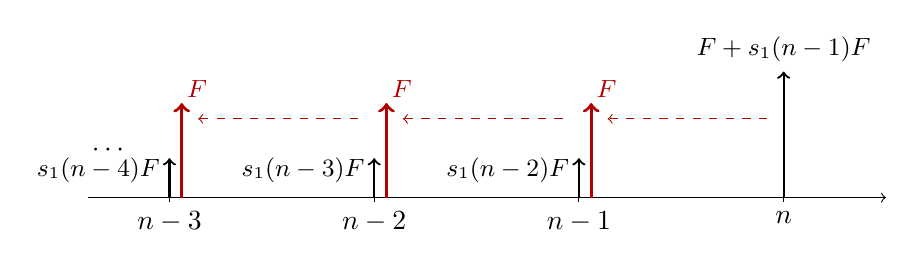
\begin{tikzpicture}[x=2.6cm]
    \draw[->] (-0.4,0) -- (3.5,0);
    \foreach \x/\l in {0/{n-3},1/{n-2},2/{n-1},3/{n}} { \draw (\x,0.06) -- (\x,-0.06) node[below] {$\l$}; }
    \draw[->, thick] (3,0) -- (3,1.6);
    \node[above] at (3,1.6) {\small $F + s_1(n-1)F$};
    \foreach \x/\c in {0/{s_1(n-4)F}, 1/{s_1(n-3)F}, 2/{s_1(n-2)F}} {
        \draw[->, thick] (\x,0) -- (\x,0.5);
        \node[left] at (\x,0.35) {\small $\c$};
        \draw[->, very thick, red!70!black] (\x+0.06,0) -- (\x+0.06,1.2) node[above right=-2pt] {\small $F$};
    }
    \foreach \x in {3,2,1} {
        \draw[->, red!70!black, dashed] (\x-0.08,1.0) -- (\x-0.86,1.0);
    }
    \node at (-0.3,0.6) {$\cdots$};
\end{tikzpicture}
\end{center}
\b{Convention}: here $PV(t)$ is the value \ul{just after} the coupon at $t$ is paid (the reset date), so it covers the cash flows at $t+1$ and later. To value at $t$, take everything received at $t+1$ (the coupon plus the value of what remains) and discount one period at the short rate in force at $t$:
\[\boxed{PV(t) = \frac{C_{t+1} + PV(t+1)}{1+s_1(t)}}\]
\aside{This differs from the running PV recursion $PV(k) = x_k + \frac{PV(k+1)}{1+f_{k,k+1}}$, which \emph{includes} the cash flow at $k$. Both are valid; they track different quantities: $PV^{\text{incl}}(t) = C_t + PV^{\text{excl}}(t)$. With the inclusive version, the floater result reads $PV(t) = C_t + F$ (still $F$ at $t=0$, where there is no coupon).}

\b{Where to start}: two equivalent choices for the end of the bond.
\begin{itemize}
    \item $PV(n) = 0$ (nothing left after maturity), with the full final cash flow $C_n = s_1(n-1)F + F$.
    \item $PV(n) = F$ (treat the face value as the bond's value at maturity), with $C_n = s_1(n-1)F$ the coupon only. This makes the induction cleanest.
\end{itemize}

Working backwards (red arrows = discount one period):
\begin{align*}
    PV(n-1) &= \frac{F + s_1(n-1)F}{1+s_1(n-1)} = \frac{F\cancel{(1+s_1(n-1))}}{\cancel{1+s_1(n-1)}} = F\\
    PV(n-2) &= \frac{s_1(n-2)F + PV(n-1)}{1+s_1(n-2)} = \frac{F + s_1(n-2)F}{1+s_1(n-2)} = F\\
    &\;\;\vdots
\end{align*}
At $n-2$, the rest of the bond acts like a lump sum of $F$ paid at $n-1$, which is exactly the situation one step later.

\b{Proof by induction} (using $PV(n) = F$):
\begin{itemize}
    \item \b{Base case}: $PV(n) = F$.
    \item \b{Inductive step}: if $PV(t+1) = F$, then
    \[PV(t) = \frac{s_1(t)F + F}{1+s_1(t)} = \frac{F\,(1+s_1(t))}{1+s_1(t)} = F.\]
\end{itemize}
Hence $PV(t) = F$ at every reset date $t = n-1, \dots, 1, 0$. $\blacksquare$

\b{Why it works}: the rate that \ul{sets the coupon} and the rate used to \ul{discount} are the same, $s_1(t)$, both fixed at time $t$. Whatever value $s_1(t)$ takes, it cancels, so you never need to know future rates (and no assumption like expectation dynamics is needed).

\begin{example}[Floater with Changing Rates]
    \b{Given}: $F = 100$, $n = 3$, yearly short rates $s_1(0) = 5\%$, $s_1(1) = 8\%$, $s_1(2) = 3\%$.
    \begin{center}
    \begin{tabular}{lccc}
        \toprule
        Time & 1 & 2 & 3\\
        \midrule
        Cash flow & 5 & 8 & $3 + 100$\\
        \bottomrule
    \end{tabular}
    \end{center}
    \b{Find}: the value at each reset date.

    \b{Solution}:
    \[PV(2) = \frac{103}{1.03} = 100, \qquad PV(1) = \frac{8 + 100}{1.08} = 100, \qquad PV(0) = \frac{5 + 100}{1.05} = \boxed{100}\]
    The rates jump around, but the value is 100 at every reset date.
\end{example}

\keypoint{A floating rate bond is worth \rb{par} ($F$) at every reset date: the coupon always exactly pays the interest for the next period.}
\aside{Consequence: a floater has very little interest-rate risk. If rates rise, the next coupon rises too and the price returns to par at the next reset, so its duration (Lecture 6) is roughly the time to the next reset. Between reset dates the price is not exactly $F$.}

\header{Example: Fishing}
Every year we decide whether to fish in a lake or not:
\begin{itemize}
    \item \b{Fish} $\rightarrow$ population stays the same. Profit is \dbb{70\% of the initial number of fish} in the lake that year.
    \item \b{Don't fish} $\rightarrow$ population doubles. Profit is 0.
\end{itemize}
Cash flows occur at the \ul{beginning} of each year, and the interest rate is 25\%. Represent the possible decisions and outcomes on a graph: horizontal = don't fish, diagonal = fish. Node labels are populations, and green numbers are the cash flows on each branch.

\begin{center}
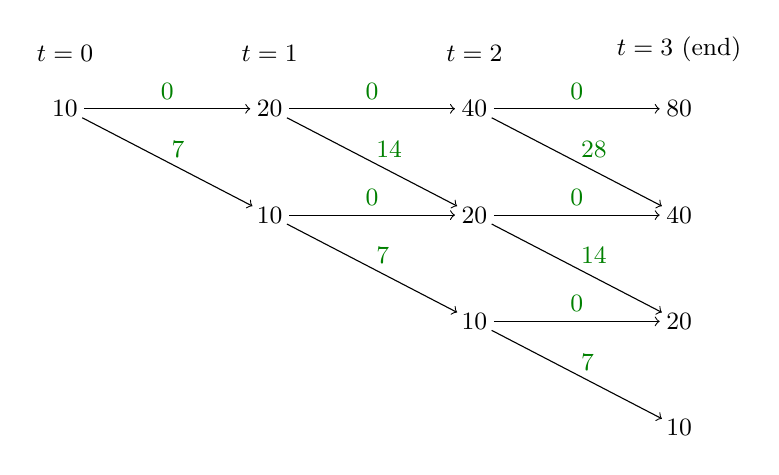
\begin{tikzpicture}[x=2.6cm, y=1.35cm]
    % populations: time t, row r (times fished) -> 10*2^(t-r)
    \foreach \t/\r/\p in {0/0/10, 1/0/20, 1/1/10, 2/0/40, 2/1/20, 2/2/10, 3/0/80, 3/1/40, 3/2/20, 3/3/10} {
        \node[circle, inner sep=1pt] (n\t\r) at (\t,-\r) {\small \p};
    }
    \foreach \t/\r/\nt/\cash in {0/0/1/7, 1/0/2/14, 1/1/2/7, 2/0/3/28, 2/1/3/14, 2/2/3/7} {
        \pgfmathtruncatemacro{\rr}{\r+1}
        \draw[->] (n\t\r) -- (n\nt\r) node[midway, above, green!50!black] {\small 0};
        \draw[->] (n\t\r) -- (n\nt\rr) node[midway, above right=-2pt, green!50!black] {\small \cash};
    }
    \node[above] at (0,0.35) {\small $t=0$};
    \node[above] at (1,0.35) {\small $t=1$};
    \node[above] at (2,0.35) {\small $t=2$};
    \node[above] at (3,0.35) {\small $t=3$ (end)};
\end{tikzpicture}
\end{center}

\b{What is the optimal fishing strategy?}
\begin{itemize}
    \item One solution: try all different fishing strategies and compare. This is a bad approach: there are too many possible paths ($2^n$ for $n$ years).
    \item A better solution: \rb{dynamic programming}, i.e.\ \ul{solve the problem backwards}.
\end{itemize}

\heading{Solving Backwards}
Dynamic programming is like running present value, except with a \dbb{decision at each step}. Let $V$ = max PV from a node, taking the better of the two branches.
\begin{enumerate}
    \item In each $\max$, the first option is \b{don't fish} and the second is \b{fish}.
    \item \b{Start at the end}: at $t = 3$ the problem is over, so every final node has $V = 0$.
    \item \b{$t = 2$} (last decision, nothing after it, so always fish):
    \[V(40) = \max(0, 28) = 28, \qquad V(20) = \max(0, 14) = 14, \qquad V(10) = \max(0, 7) = 7\]
    \item \b{$t = 1$}: each option is the cash flow now plus the discounted value of where it takes you:
    \begin{align*}
        V(20) &= \max\left(0 + \tfrac{28}{1.25},\; 14 + \tfrac{14}{1.25}\right) = \max(22.4,\ 25.2) = 25.2 \quad \text{(fish)}\\
        V(10) &= \max\left(0 + \tfrac{14}{1.25},\; 7 + \tfrac{7}{1.25}\right) = \max(11.2,\ 12.6) = 12.6 \quad \text{(fish)}
    \end{align*}
    \item \b{$t = 0$}:
    \[V(10) = \max\left(0 + \tfrac{25.2}{1.25},\; 7 + \tfrac{12.6}{1.25}\right) = \max(20.16,\ 17.08) = \boxed{20.16} \quad \text{(don't fish)}\]
\end{enumerate}

\begin{center}
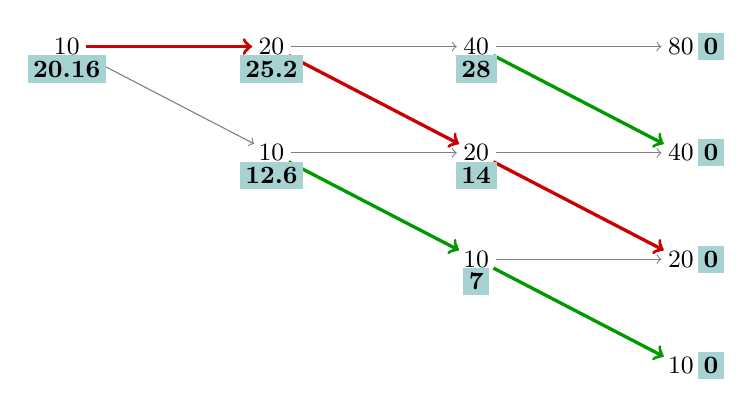
\begin{tikzpicture}[x=2.6cm, y=1.35cm]
    \tikzset{vbox/.style={fill=teal!35, font=\small\bfseries, inner sep=2pt}}
    \foreach \t/\r/\p in {0/0/10, 1/0/20, 1/1/10, 2/0/40, 2/1/20, 2/2/10, 3/0/80, 3/1/40, 3/2/20, 3/3/10} {
        \node[circle, inner sep=1pt] (n\t\r) at (\t,-\r) {\small \p};
    }
    \foreach \t/\r/\nt in {0/0/1, 1/0/2, 1/1/2, 2/0/3, 2/1/3, 2/2/3} {
        \pgfmathtruncatemacro{\rr}{\r+1}
        \draw[->, gray] (n\t\r) -- (n\nt\r);
        \draw[->, gray] (n\t\r) -- (n\nt\rr);
    }
    % optimal decision at each node (green), optimal path from the start (red)
    \draw[->, very thick, green!60!black] (n20) -- (n31);
    \draw[->, very thick, green!60!black] (n22) -- (n33);
    \draw[->, very thick, green!60!black] (n11) -- (n22);
    \draw[->, very thick, red!80!black] (n00) -- (n10);
    \draw[->, very thick, red!80!black] (n10) -- (n21);
    \draw[->, very thick, red!80!black] (n21) -- (n32);
    \foreach \t/\r/\v in {0/0/20.16, 1/0/25.2, 1/1/12.6, 2/0/28, 2/1/14, 2/2/7} {
        \node[vbox, below=3pt] at (n\t\r) {\v};
    }
    \foreach \r in {0,1,2,3} { \node[vbox, right=6pt] at (n3\r) {0}; }
\end{tikzpicture}
\end{center}
\keypoint{Optimal strategy (red path): \rb{don't fish} in year 0, then \rb{fish} in years 1 and 2, for a max PV of $0 + \frac{14}{1.25} + \frac{14}{1.25^2} = 20.16$.}
Green arrows show the best decision at every other node, so the solution tells you what to do from \ul{any} state, not just the path you expect to follow.
\\Note: if the interest rate weren't constant, we would use the \dbb{forward short rates} to discount.

\header{The Basic Recursion}
\b{Dynamic decisions}: problems where cash flows depend on decisions that will be made at future times. These are similar to running present value calculations, except we have a decision to make at each time.
\keypoint{Always remember to \rb{``solve the problem backwards''}.}

\begin{definition}[\rb{Value Function}]
    $V(x,t)$ is the \dbb{maximum present value} given that you are at the current state $x$ and time $t$.
\end{definition}
The maximum is achieved by maximizing \{\db{next step + the optimum from where that takes you}\}:
\[\boxed{V(x,t) = \max_i\left[c_i + \tfrac{1}{1+r}V(y_i, t+\Delta t)\right]}\]
\begin{itemize}
    \item $V(x,t)$: the optimum from state $x$.
    \item $c_i$: the next step, i.e.\ the cash flow (at the beginning of the period) from choice $i$.
    \item $\frac{1}{1+r}$: the discount.
    \item $V(y_i, t+\Delta t)$: the optimum PV from the state $y_i$ that choice $i$ takes you to.
\end{itemize}

\begin{center}
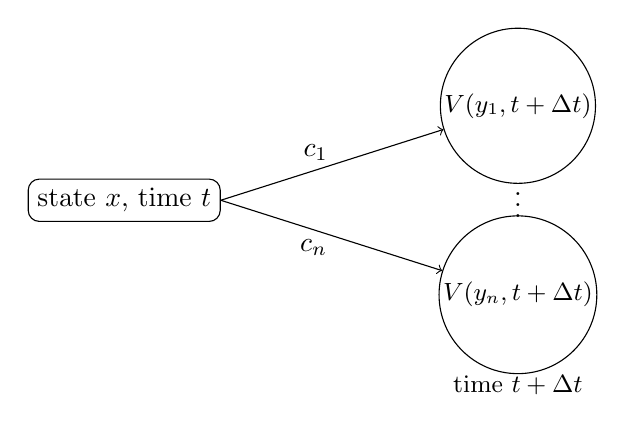
\begin{tikzpicture}
    \node[draw, rounded corners] (x) at (0,0) {state $x$, time $t$};
    \node[draw, circle, inner sep=1pt] (y1) at (5,1.2) {\small $V(y_1, t+\Delta t)$};
    \node[draw, circle, inner sep=1pt] (yn) at (5,-1.2) {\small $V(y_n, t+\Delta t)$};
    \node at (5,0.05) {$\vdots$};
    \draw[->] (x.east) -- (y1) node[midway, above left=-2pt] {$c_1$};
    \draw[->] (x.east) -- (yn) node[midway, below left=-2pt] {$c_n$};
    \node[below] at (5,-2.1) {\small time $t + \Delta t$};
\end{tikzpicture}
\end{center}
This recursion is started \ul{at the end} and goes \ul{backwards}.

\header{Including Probability}
When things are uncertain, we often want to maximize an \dbb{expected value}. Then $V(x,t)$ is the maximum \rb{expected} present value given you are at state $x$ and time $t$:
\[V(x,t) = \max\left[E(PV \mid x,t)\right]\]
and the recursion is
\[\boxed{V(x,t) = \max_i\left[E\left[c_i + \tfrac{1}{1+r}V(y_i, t+\Delta t) \;\middle|\; x,t\right]\right]}\]
\begin{center}
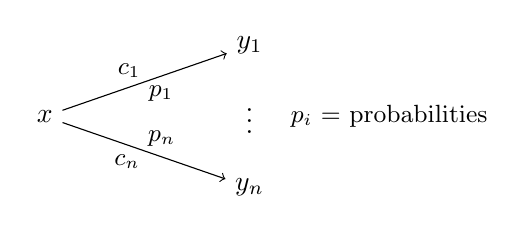
\begin{tikzpicture}
    \node (x) at (0,0) {$x$};
    \node (y1) at (2.6,0.9) {$y_1$};
    \node (yn) at (2.6,-0.9) {$y_n$};
    \node at (2.6,0.05) {$\vdots$};
    \draw[->] (x) -- (y1) node[midway, above left=-2pt] {\small $c_1$} node[midway, below right=-2pt] {\small $p_1$};
    \draw[->] (x) -- (yn) node[midway, below left=-2pt] {\small $c_n$} node[midway, above right=-2pt] {\small $p_n$};
    \node[right] at (3,0) {\small $p_i$ = probabilities};
\end{tikzpicture}
\end{center}
Once again, we always \ul{start at the end}.

\header{Example: Rolling a Die}
You have \dbb{3 chances} to roll a die. After each roll you can either \b{stop} and receive a dollar amount equal to that roll, or \b{discard} that roll and roll again. How much would you pay to play this? When should you say ``stop''? (No discounting.)

Let $V_t$ be the value after seeing roll $t$. On each roll, compare stopping (take the roll) with continuing (expected value of the next roll's $V$):
\[V_t = \max\left[\text{roll},\; E[V_{t+1}]\right]\]
\begin{itemize}
    \item \b{Roll 3} (last roll, must stop): $V_3 = \text{roll}$, so $E[V_3] = \frac{1+2+3+4+5+6}{6} = 3.5$.
    \item \b{Roll 2}: stop if the roll beats 3.5, i.e.\ on \dbb{4, 5, 6}:
    \[E[V_2] = \frac{3.5 + 3.5 + 3.5 + 4 + 5 + 6}{6} = 4.25\]
    \item \b{Roll 1}: stop if the roll beats 4.25, i.e.\ on \dbb{5, 6}:
    \[E[V_1] = \frac{4.25 + 4.25 + 4.25 + 4.25 + 5 + 6}{6} = 4.667\]
\end{itemize}
\begin{center}
\begin{tabular}{cccc}
    \toprule
    Roll outcome & Roll 1: $V_1$ & Roll 2: $V_2$ & Roll 3: $V_3$\\
    \midrule
    6 & \textcolor{red!70!black}{$\bullet$} 6 & \textcolor{red!70!black}{$\bullet$} 6 & \textcolor{red!70!black}{$\bullet$} 6\\
    5 & \textcolor{red!70!black}{$\bullet$} 5 & \textcolor{red!70!black}{$\bullet$} 5 & \textcolor{red!70!black}{$\bullet$} 5\\
    4 & 4.25 & \textcolor{red!70!black}{$\bullet$} 4 & \textcolor{red!70!black}{$\bullet$} 4\\
    3 & 4.25 & 3.5 & \textcolor{red!70!black}{$\bullet$} 3\\
    2 & 4.25 & 3.5 & \textcolor{red!70!black}{$\bullet$} 2\\
    1 & 4.25 & 3.5 & \textcolor{red!70!black}{$\bullet$} 1\\
    \midrule
    $E[V_t]$ & \fbox{4.667} & 4.25 & 3.5\\
    \bottomrule
\end{tabular}
\\[2pt]{\small \textcolor{red!70!black}{$\bullet$} = stop nodes}
\end{center}
\keypoint{The game is worth \rb{\$4.67}: on roll 1 stop on 5 or 6, on roll 2 stop on 4, 5 or 6, and on roll 3 take whatever you get.}
(The slide's worked figures, 3.5714, 4.24488 and 4.6034, don't match this recursion. The values here agree with the spreadsheet below, and the stop rules are the same either way.)

\begin{example}[More Rolls]
    The same recursion with up to 10 rolls, $E_n = \frac{1}{6}\sum_{i=1}^{6}\max(i, E_{n-1})$ with $E_0 = 0$:
    \begin{center}
    \begin{tabular}{lcccccccccc}
        \toprule
        Rolls left & 1 & 2 & 3 & 4 & 5 & 6 & 7 & 8 & 9 & 10\\
        \midrule
        Value & 3.5 & 4.25 & 4.667 & 4.944 & 5.130 & 5.275 & 5.396 & 5.496 & 5.580 & 5.650\\
        Stop on & any & $\geq 4$ & $\geq 5$ & $\geq 5$ & $\geq 5$ & 6 & 6 & 6 & 6 & 6\\
        \bottomrule
    \end{tabular}
    \end{center}
    ``Stop on'' is the rule for the current roll: stop if the roll beats the value of the game with one fewer roll left. With more rolls left you can afford to be pickier, and the value creeps up towards 6.
\end{example}

\header{Example: The Complexico Mine}
You consider leasing a gold mine which is approaching depletion.
\begin{itemize}
    \item If $x$ is the amount of gold remaining at the beginning of a year, the cost to extract $z < x$ ounces that year is $\dfrac{500z^2}{x}$.
    \item Current gold remaining: $x = 50{,}000$ ounces. Price of gold: $g = \$400$/ounce. Interest rate: 10\%.
\end{itemize}
\keypoint{Q: How much is a \rb{10 year lease} worth?}

We must determine the optimal way to mine over the 10 year lease. This time we are \ul{not on a finite graph}: the amount of gold in the mine is a \dbb{continuous variable}. We still solve the problem backwards using dynamic programming.

\begin{center}
\begin{tikzpicture}
    \draw[->] (0,-0.3) -- (0,2.4) node[above] {\small gold left};
    \draw[thick, |->] (0.3,0) -- (9.4,0);
    \foreach \x/\l in {0.3/0, 1.3/1, 6.2/8, 7.4/9, 8.6/10} { \draw[thick] (\x,0.1) -- (\x,-0.1) node[below] {\l}; }
    \node at (3.75,0.5) {$\cdots$};
    \draw[dotted] (7.4,0.2) -- (7.4,2.2);
    \draw[dotted] (8.6,0.2) -- (8.6,2.2);
    \node[left] at (7.4,1.8) {$x$};
    \foreach \y in {1.8,1.5,1.2,0.9,0.6} { \draw[->] (7.45,1.8) -- (8.55,\y); }
    \node[above] at (8.6,2.2) {\small $V_{10}(x) = 0$};
\end{tikzpicture}
\end{center}
Each arrow is a different choice of how much gold $z$ to remove that year.

Assume cash flows occur at the beginning of the year. Let $V_t(x)$ be the optimal value of the lease at time $t$ given that $x$ is the amount of gold left in the mine.

\heading{Step 1: The End}
At time 10 the lease is up, so $V_{10}(x) = 0$.

\heading{Step 2: $V_9(x)$}
Let $z_9$ be the amount of gold removed in year 9. The cash flow at time 9 is
\[\underbrace{400z_9}_{\text{revenue}} - \underbrace{500\frac{z_9^2}{x}}_{\text{cost}}\]
Dynamic programming says
\[V_9(x) = \max_{z_9}\Bigg(\underbrace{400z_9 - 500\frac{z_9^2}{x}}_{\text{cash flow at time 9}} + \underbrace{\frac{1}{1.1}V_{10}(x - z_9)}_{=\,0}\Bigg) = \max_{z_9}\left(400z_9 - 500\frac{z_9^2}{x}\right)\]
Maximize by setting the derivative equal to zero:
\[400 - \frac{1000z_9}{x} = 0 \quad \Rightarrow \quad z_9 = \frac{4x}{10}\]
Plugging back in: $V_9(x) = 400\cdot\frac{4x}{10} - 500\cdot\frac{16x^2/100}{x} = 160x - 80x$, so
\[\boxed{V_9(x) = 80x = K_9x, \quad K_9 = 80}\]

\heading{Step 3: $V_8(x)$}
Let $z_8$ be the amount removed in year 8. After year 8, $x - z_8$ is left, and we already know $V_9(x) = K_9x$:
\[V_8(x) = \max_{z_8}\left(400z_8 - 500\frac{z_8^2}{x} + \frac{1}{1.1}V_9(x - z_8)\right) = \max_{z_8}\left(400z_8 - 500\frac{z_8^2}{x} + \frac{1}{1.1}K_9(x - z_8)\right)\]
Setting the derivative to zero:
\[400 - \frac{1000z_8}{x} - \frac{K_9}{1.1} = 0 \quad \Rightarrow \quad z_8 = \frac{\left(400 - \frac{1}{1.1}K_9\right)x}{1000}\]
Plugging back in (with $a = 400 - \frac{1}{1.1}K_9$, the first two terms give $\frac{a^2x}{1000} - \frac{a^2x}{2000} = \frac{a^2x}{2000}$):
\[\boxed{V_8(x) = \left[\frac{\left(400 - \frac{1}{1.1}K_9\right)^2}{2000} + \frac{1}{1.1}K_9\right]x = K_8x}\]

\heading{Step 4: Continue Backwards}
Every step has the same form, so $V_7(x) = K_7x$, $V_6(x) = K_6x$, $\dots$, $V_0(x) = K_0x$, where
\[\boxed{K_j = \frac{\left(400 - \frac{1}{1.1}K_{j+1}\right)^2}{2000} + \frac{1}{1.1}K_{j+1}, \qquad K_{10} = 0}\]
with optimal extraction $z_j = \frac{\left(400 - \frac{1}{1.1}K_{j+1}\right)x}{1000}$, which is always less than $x$, as required.
\keypoint{The value of the 10 year lease is $V_0(50{,}000) = K_0 \cdot 50{,}000$.}

\begin{example}[Complexico Mine Spreadsheet]
    The slide's spreadsheet uses an interest rate of \dbb{5\%} (replace $1.1$ by $1.05$ above):
    \begin{center}
    \setlength{\tabcolsep}{4pt}
    \begin{tabular}{lccccccccccc}
        \toprule
        Time & 0 & 1 & 2 & 3 & 4 & 5 & 6 & 7 & 8 & 9 & 10\\
        \midrule
        $K$ & 239.19 & 234.82 & 229.23 & 222.03 & 212.66 & 200.32 & 183.75 & 161.00 & 128.62 & 80 & 0\\
        \bottomrule
    \end{tabular}
    \end{center}
    \[V_0(50{,}000) = 239.191274 \times 50{,}000 = \boxed{\$11{,}959{,}563.70}\]
    At the question's \dbb{10\%} rate, the same recursion gives $K_8 = 126.28$, $K_0 = 213.81$, and a lease value of about \$10,690,747. It is lower, since future gold is discounted more heavily.
\end{example}
